% !TeX program = pdflatex
% !TeX encoding = utf8
% !TeX spellcheck = uk_UA
% !BIB program = bibtex8

\documentclass{LabWorkTemplate}
\usetikzlibrary{math}
%============================================= Заголовок документу ====================================================%
\work{3}
\title{Кільця Ньютона}

\author{Тор А.~В.}{}
\author{Другий А.~В.}{}

\group{ФФ-93}

\abstract{Ознайомлення з явищем інтерференції в тонких плівках (смуги рівної товщини) на прикладі кілець Ньютона і з методикою інтерференційних вимірювань кривизни скляної поверхні.}
\keywords{когерентність, інтерференція світла, оптична довжина ходу хвилі, інтерференційна схема}
%======================================================================================================================%

\begin{document}
\writedatatofile{\jobname}
\maketitle



\section{Теоретичне підґрунтя}

Кільця Ньютона утворюються при інтерференції світлових хвиль, відбитих від границь тонкого повітряного прошарку, який знаходиться між опуклою поверхнею лінзи і плоскою скляною пластинкою (рис.~\ref{pic1}). Спостереження ведеться у відбитому світлі.

\begin{wrapfigure}{r}{0.4\linewidth}
	\begin{center}
		\begin{tikzpicture}[decoration={ markings,  mark=at position 0.5 with {\arrow{stealth}}},]
%    	\draw (-3,-3) to [grid with coordinates] (3,3);
        \fill[cyan, top color = cyan!50,  bottom color = cyan!50, middle color = white, draw=cyan] (-3,-0.25) rectangle (3,0.25);
%        \draw[dashed] (0,7.5) circle (7);
        \fill[cyan, top color = cyan!50,  bottom color = cyan!50, middle color = white, draw=cyan] (0,7.5) ++(244:7) arc (244:296:7) -- cycle;
        \draw (0,7.5) -- node[right] {$R$}++(287:7);
        \draw (0,7.5) -- ++(270:8.3);
        \draw [stealth reversed-stealth reversed] (2.6,0.9) -- node [right] {$d$} (2.6,0.4);
        \draw [stealth reversed-stealth reversed] (2,0.6)    --  node [left] {$d_0$} (2,0.15);
        \draw [thin, dashed] (-3,0.8) -- (3,0.8);
        \draw [thin, dashed] (0,0.50) -- (3,0.50);
        \draw (-2,0.8) -- ++(0,-1.6);
        \draw [latex-latex] (-2,-0.6) -- node[below] {$r_m$} (0,-0.6);
        \draw [red, postaction={decorate}] (-2.8, 4) node[left, black] {$1$} -- (-2.8,1.08) ;
        \draw [red, -stealth] (-2.8,1.08) -- (-2.2,0.25) -- (-2,0.8) -- (-1.2,1.6) node[above right, black] {$2'$} node[above left, black] {$1'$};
%        \draw[-stealth, red] (-2.8,1.08) -- (-2.5, 1.6);
        \draw [red, postaction={decorate}] (-2, 4) node[right, black] {$2$} -- (-2,0.8);
	\end{tikzpicture}
	\end{center}
	\caption{Утворення кілець Ньютона}
	\label{pic1}
\end{wrapfigure}
Нехай на систему згори падає монохроматичний паралельний пучок променів. Частина променів (промінь 1 на рис.~\ref{pic1} ) відбивається від верхнього краю пластини, а інша частина(промінь 2 на рис.~\ref{pic1}) від нижнього краю лінзи.

Промені $1'$ та $2'$ когерентні,  але між ними виникає різниця ходу. Роль тонкої плівки виконує повітряний проміжок між пластиною та лінзою.Нехай на систему згори  падає монохроматичний паралельний пучок променів. Частина променів (промінь 1 на рис.~\ref{pic1}) відбивається від верхнього краю пластини, а інша частина(промінь $2$ на рис.~\ref{pic1}) від нижнього краю лінзи. Промені $1'$ та $2'$ когерентні,  але між ними виникає різниця ходу. В першому наближені, як що знехтувати невеликим нахилом променів у повітряному зазорі, геометрична різниця ходу дорівнює:
\begin{equation}
\delta' =2(d+d_{0})
\end{equation}
де $d_{0}$~--- товщина зазору в місці контакту лінзи та пластини, яка може бути як додатною, наприклад, за наявності часток пилу між лінзою та пластиною, який викликає деформацію; $d_{0}+d$~--- товщина повітряного зазору на відстані $r_m$ від центру лінзи. Для того, щоб визначити повну  різницю ходу $d$  треба прийняти до уваги зміну фаз світлової хвилі під час відбиття від гранці поділу скло-повітря,коли показник заломлення першого середовища більше за показник заломлення другого, та під час відбиття від гранці повітря-скло, коли навпаки показник заломлення першого середовища менше за показник заломлення другого. Відомо, що для електричного вектора у першому випадку відбиття відбувається  без зміни фаз, а в другому призводить до зміни  фаз на $\pi$; фаза магнітного вектора, навпаки,змінюється на $\pi$ тільки під час першого відбиття. Таким чином, промені 1 і 2 набувають різниці фаз $\pi$, що відповідає додатковій різниці ходу $\lambda/2$, а повна різниця ходу:

\begin{equation}
\delta =2(d+d_{0})+\lambda/2.
\end{equation}

Якщо форма лінзи близька до сферичної з радіусом кривизни $R \gg r_m$, то геометричного міркувань $r^2_m = 2Rd $, і
\begin{equation}
\delta=r^2_m/R+2d_{0}+\lambda/2.
\end{equation}

Якщо повна різниця ходу дорівнює $\lambda(m+1/2)$, то промені 1 і 2 гаситимуть один одного і спостерігатимуться темні плями(кільця). Радіус цих кілець $r_\text{тем}$ легко розрахувати за формулою:
\begin{equation}
\label{rdark}
r_\text{тем}^2=R(\lambda m-2d_{0})
\end{equation}

Аналогічно, для радіуса світлих кілець $r_\text{світ}$ маємо:

\begin{equation}
\label{rlight}
r_\text{світ}^2=R(\lambda m-2d_{0}-\lambda/2)
\end{equation}

Отже, за графіком залежності $r^2_m$ від номеру кільця можна визначити радіус кривизни лінзи, а також величину проміжку в місці контакту.

\section{Експерементальні подробиці}


В даній лабораторній роботі кільця Ньютона досліджується за допомогою мікроскопа МБС-10. На столику мікроскопа розташоване держак, на якому розміщується досліджувана лінза з пластиною. В одному з окулярів мікроскопа встановлюється освітювач, що генерує пучок променів, паралельних тим, що падають в околі спостерігача. Для монохроматизації пучка перед освітлювачем встановлюють фільтр. В комплект входять 7 фільтрів, що створюють  монохроматичні пучки, довжини хвилі яких наведені в таблиці~\ref{WaveLength}.

\begin{wraptable}[10]{O}{0.5\linewidth}
	\centering
	\begin{tabular}{lc}
		\toprule
		Колір                          & Довжина хвилі $\lambda$,~нм \\ \midrule
		\rowcolor{violet!10}Фіолетовий &             $ 404 \pm 10$             \\
		\rowcolor{blue!10}Синій        &             $ 434 \pm 10$             \\
		\rowcolor{cyan!10}Блакитний    &             $ 486 \pm 10 $             \\
		\rowcolor{green!10}Зелений     &             $ 546 \pm 10 $             \\
		\rowcolor{yellow!10}Жовтий     &             $ 586 \pm 10 $             \\
		\rowcolor{orange!10}Оранжевий  &             $ 656 \pm 10 $             \\
		\rowcolor{red!10}Червоний      &             $ 706 \pm 10 $             \\ \bottomrule
	\end{tabular}
	\caption{Довжини хвиль}
	\label{WaveLength}
\end{wraptable}
На початку експерименту рекомендуються знайти кільця Ньютона в білому світлі (без фільтра) і сфокусувати мікроскоп під своє око. Перехрестя шкал мікроскопа повинно проходити через центр кілець. Після цього можна встановити фільтр і переходити до безпосередніх вимірювань радіусу кілець. Для вимірювань  на окулярі мікроскопа нанесено спеціальну шкалу з поділками. Ціну поділки для кожного значення збільшення вказано в інструкції до мікроскопа.

Вимірювати радіус кілець слід від центру системи до середини кільця. Для збільшення точності рекомендуємо після першої серії вимірів із заданим фільтром повернути лінзу на $90^\circ$ навколо вертикальної осі  і повторити виміри. Якщо робота виконується двома студентами, то рекомендуємо провести виміри кожному з студентів, а потім порівняти й усереднити одержані результати.

\newpage
\section{Результи вимiрювань та обробка експериментальних даних}

Завдяки мікроскопу спостерігаються кільця Ньютона у відбитому світлі лампи розжарення при $\sim 70$~кратному збільшенні.

Встановивши відповідний світлофільтр (монохроматор) можна спостерігати кільця Ньютона в монохроматичному світлі.

Завдяки шкалі (ціна поділки $2.5 \cdot 10^{-2}$~мм/поділку), нанесеній на скло окуляра вимірювався діаметр світлих кілець.

% =========================================
\pgfplotstableread{red.dat}\RedTable
\pgfplotstableread{Blue.dat}\BlueTable
\pgfplotstableread{yellow.dat}\YellowTable
% =========================================

\pgfplotstablecreatecol[
	create col/expr={\thisrow{r}^2},
]{rsqr}\RedTable
\pgfplotstablecreatecol[
	create col/expr={\thisrow{rError}^2},
]{rsqrError}\RedTable

\pgfplotstablecreatecol[
	create col/expr={\thisrow{r}^2},
]{rsqr}\BlueTable
\pgfplotstablecreatecol[
	create col/expr={\thisrow{rError}^2},
]{rsqrError}\BlueTable


\pgfplotstablecreatecol[
	create col/expr={\thisrow{r}^2},
]{rsqr}\YellowTable
\pgfplotstablecreatecol[
	create col/expr={\thisrow{rError}^2},
]{rsqrError}\YellowTable

% =========================================

%---------------------------------------------------------
\begin{minipage}{0.4\linewidth}\centering
   \begin{center}
        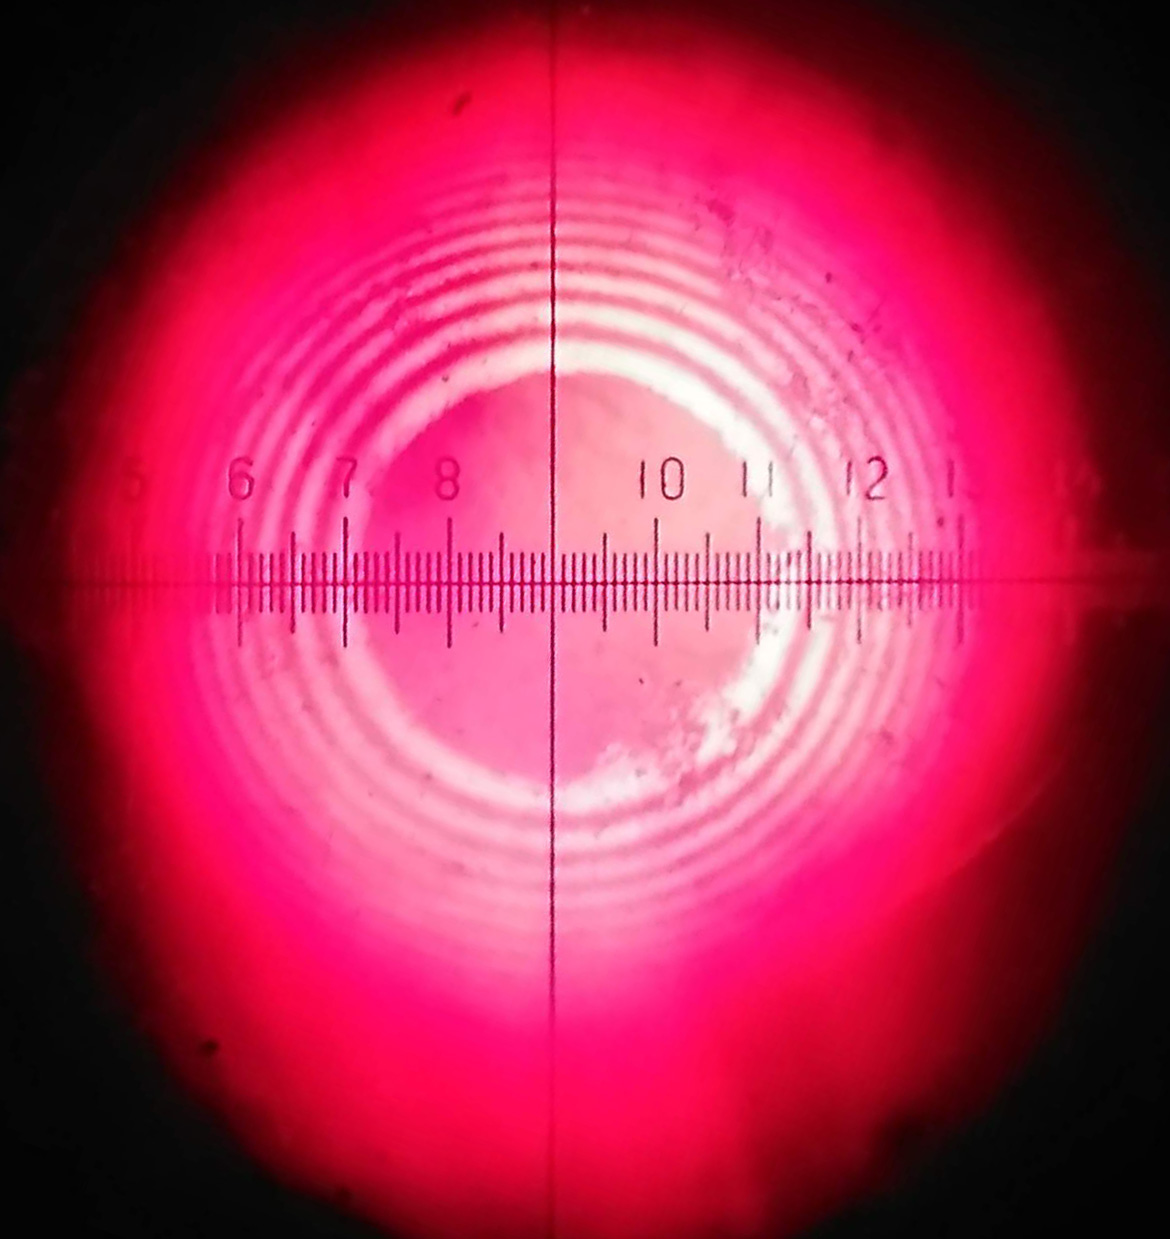
\includegraphics[width=0.95\linewidth]{Red}
    \label{fig:Red}
    \end{center}
\end{minipage}%
\qquad%---------------------------------------------------------
\begin{minipage}{0.4\linewidth}\centering
               Експериментальні дані для червоного кольору
            \pgfplotstabletypeset[
            columns={N,r,rError,rsqr},
            columns/N/.style={int detect, column type=r, column name=$m$},
            columns/r/.style={column type=c, column name={$r$, мм}},
            columns/rError/.style={column type=c, column name={$\pm\Delta r$, мм}},
            columns/rsqr/.style={column type=c, column name={$r^2$, мм$^2$}},
            every head row/.style={
            before row=\toprule,after row=\midrule},
            every last row/.style={
            after row=\bottomrule},
             fixed, fixed zerofill,
            ]
            \RedTable
\end{minipage}

%---------------------------------------------------------
\begin{minipage}{0.4\linewidth}\centering
   \begin{center}
        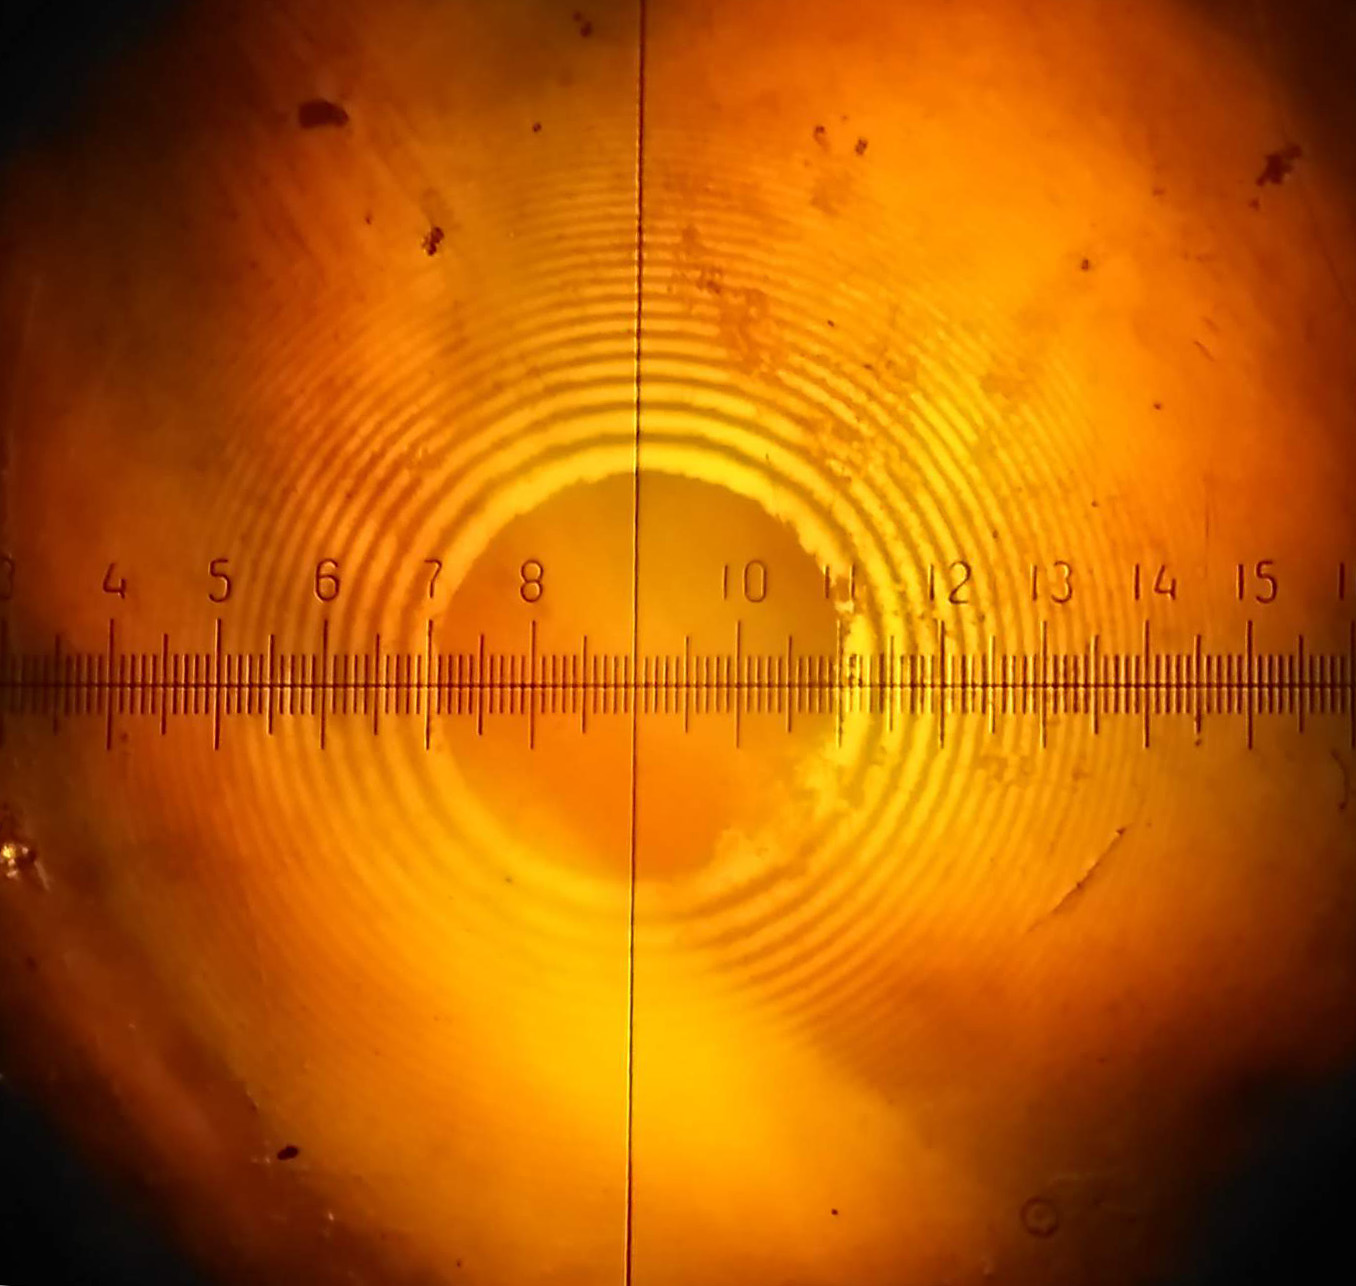
\includegraphics[width=0.95\linewidth]{Yellow}
    \label{fig:Yellow}
    \end{center}
\end{minipage}%
\qquad%---------------------------------------------------------
\begin{minipage}{0.4\linewidth}\centering
               Експериментальні дані для жовтого кольору
            \pgfplotstabletypeset[
            columns={N,r,rError,rsqr},
            columns/N/.style={int detect, column type=r, column name=$m$},
            columns/r/.style={column type=c, column name={$r$, мм}},
            columns/rError/.style={column type=c, column name={$\pm\Delta r$, мм}},
            columns/rsqr/.style={column type=c, column name={$r^2$, мм$^2$}},
            every head row/.style={
            before row=\toprule,after row=\midrule},
            every last row/.style={
            after row=\bottomrule},
             fixed, fixed zerofill,
            ]
            \YellowTable
\end{minipage}


%---------------------------------------------------------
\begin{minipage}{0.4\linewidth}\centering
   \begin{center}
        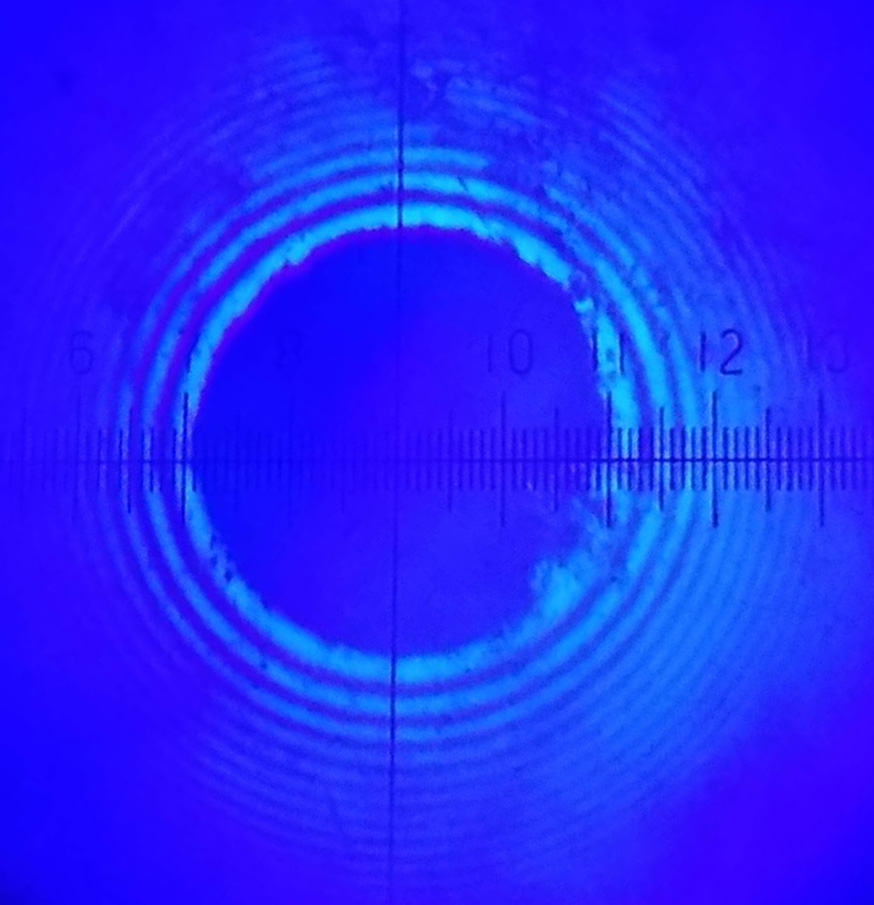
\includegraphics[width=0.95\linewidth]{Blue}
    \label{fig:Blue}
    \end{center}
\end{minipage}%
\qquad%---------------------------------------------------------
\begin{minipage}{0.4\linewidth}\centering
               Експериментальні дані для синього кольору
            \pgfplotstabletypeset[
            columns={N,r,rError,rsqr},
            columns/N/.style={int detect, column type=r, column name=$m$},
            columns/r/.style={column type=c, column name={$r$, мм}},
            columns/rError/.style={column type=c, column name={$\pm\Delta r$, мм}},
            columns/rsqr/.style={column type=c, column name={$r^2$, мм$^2$}},
            every head row/.style={
            before row=\toprule,after row=\midrule},
            every last row/.style={
            after row=\bottomrule},
             fixed, fixed zerofill,
            ]
            \BlueTable
\end{minipage}

\begin{center}
	\begin{tikzpicture}[
			declare function={
					lambdar  = 706e-6;
                    lambday  = 585e-6;
                    lambdab  = 404e-6;
				},
		]


		\begin{axis}[legend style={at={(current axis.north west), font=\footnotesize},anchor=north west},
				% === Налаштування сітки ===
				grid = both,
				major grid style={line width=.6pt,draw=brown!60},
				minor tick num = 9,
				minor grid style = {line width=.1pt,draw=brown!20},
%				axis lines = middle,
%				axis line style={-stealth},
				xlabel={$m$},
				ylabel={$r^2$, мм$^2$},
%				ylabel style={above right},
				every tick/.style={black},
				extra x ticks={1, 2, 3, 4, 5},
				xtick = {},
                xticklabels={},
				ytick = {},
				xmin = 1.5,
				xmax =  5.5,
				ymin = 0.3,
				ymax =  0.75,
				width=1\linewidth,
				height=0.5\textheight,
			]


			\addplot[
				red,
				only marks,
				error bars/.cd,
				y dir = both,  y explicit,
			]
			table[
					x=N,
					y expr={\thisrow{rsqr}},
					y error = rsqrError,
				]\RedTable;


			\addlegendentry{Червоний}


			\addplot[red, dashed,
			]
			table[x=N, y={create col/linear regression={y = rsqr}}]\RedTable;
			\xdef\slopeR{\pgfplotstableregressiona}
			\xdef\ycepteR{\pgfplotstableregressionb}

			\addlegendentry{
				$\pgfmathprintnumber{\slopeR}m \pgfmathprintnumber[print sign]{\ycepteR}$ ---лінійна апроксимація
			}
%-------------------------------------------------------

			\addplot[
				brown,
				only marks,
				error bars/.cd,
				y dir = both,  y explicit,
			]
			table[
					x=N,
					y expr={\thisrow{rsqr}},
					y error = rsqrError,
				]\YellowTable;

            \addlegendentry{Жовтий}

			\addplot[red, dashed,
			]
			table[x=N, y={create col/linear regression={y = rsqr}}]\YellowTable;
			\xdef\slopeY{\pgfplotstableregressiona}
			\xdef\ycepteY{\pgfplotstableregressionb}

			\addlegendentry{
				$\pgfmathprintnumber{\slopeY} m \pgfmathprintnumber[print sign]{\ycepteY}$ ---лінійна апроксимація
			}

%-------------------------------------------------------

			\addplot[
				blue,
				only marks,
				error bars/.cd,
				y dir = both,  y explicit,
			]
			table[
					x=N,
					y expr={\thisrow{rsqr}},
					y error = rsqrError,
				]\BlueTable;

            \addlegendentry{Синій}

			\addplot[blue, dashed,
			]
			table[x=N, y={create col/linear regression={y = rsqr}}]\BlueTable;
			\xdef\slopeB{\pgfplotstableregressiona}
			\xdef\ycepteB{\pgfplotstableregressionb}

			\addlegendentry{
				$\pgfmathprintnumber{\slopeB} m \pgfmathprintnumber[print sign]{\ycepteB}$ ---лінійна апроксимація
			}

% ----------------------------------------------------------------------------------------------------------
			\node[anchor = south east, text width=5cm, font=\footnotesize, fill=white, draw=black] at (current axis.south east) {
					$\lambda_{Red} = \pgfmathprintnumberFE[custom exponent=-6,precision=2]{lambdar}$~мм \\
					$R = \pgfmathprintnumberFE[custom exponent=0, precision=1, fixed zerofill]{\slopeR/lambdar/10} \pm
                    \pgfmathprintnumberFE[custom exponent=0,precision=1]{1/lambdar/10*sqrt(0.005^2+\slopeR^2*1e-10/lambdar^2)}$~см \\
                    \hrulefill\\
					$\lambda_{Yellow} = \pgfmathprintnumberFE[custom exponent=-6,precision=2]{lambday}$~мм \\
					$R = \pgfmathprintnumberFE[custom exponent=0, precision=1, fixed zerofill]{\slopeY/lambday/10} \pm
                    \pgfmathprintnumberFE[custom exponent=0,precision=1]{1/lambday/10*sqrt(0.0032^2+\slopeY^2*1e-10/lambday^2)}$~см \\
                    \hrulefill \\
					$\lambda_{Blue} = \pgfmathprintnumberFE[custom exponent=-6,precision=2]{lambdab}$~мм \\
					$R = \pgfmathprintnumberFE[custom exponent=0, precision=1, fixed zerofill]{\slopeB/lambdab/10} \pm
                    \pgfmathprintnumberFE[custom exponent=0,precision=1]{1/lambdab/10*sqrt(0.005^2+\slopeB^2*1e-10/lambdab^2)}$~см \\
			};
		\end{axis}
	\end{tikzpicture}
\captionof{figure}{Результати експерименту та розраховане значення радіуса кривизни лінзи $R$}
\end{center}
%---------------------------------------------------------
\end{document}
